\chapter{Anforderungsanalyse} 
\label{chapter:Kapitel3}
\lhead{Kapitel 3. \emph{Anforderungsanalyse}}  

Das Ziel der vorliegenden Arbeit ist die prototypische Implementierung einer leichtgewichtigen Personal Learning Environment mit Offlinefähigkeiten auf Basis aktueller Technologien. In Abschnitt \ref{section:anwendungsfaelle} werden typische Anwendungsfälle beschrieben, die für ein solches System umgesetzt werden müssen. Auf Basis dieser Anwendungsfälle werden die funktionalen Anforderungen an das System abgeleitet. In Abschnitt \ref{section:nichtfunktionale_anforderunge} werden anschließend werden auf Basis von anderen Randbedingungen weitere (nichtfunktionale) Anforderungen definiert.

\section{Anwendungsfälle/Funktionale Anforderungen}\label{section:anwendungsfaelle}
\begin{figure}[h]
  \centering
  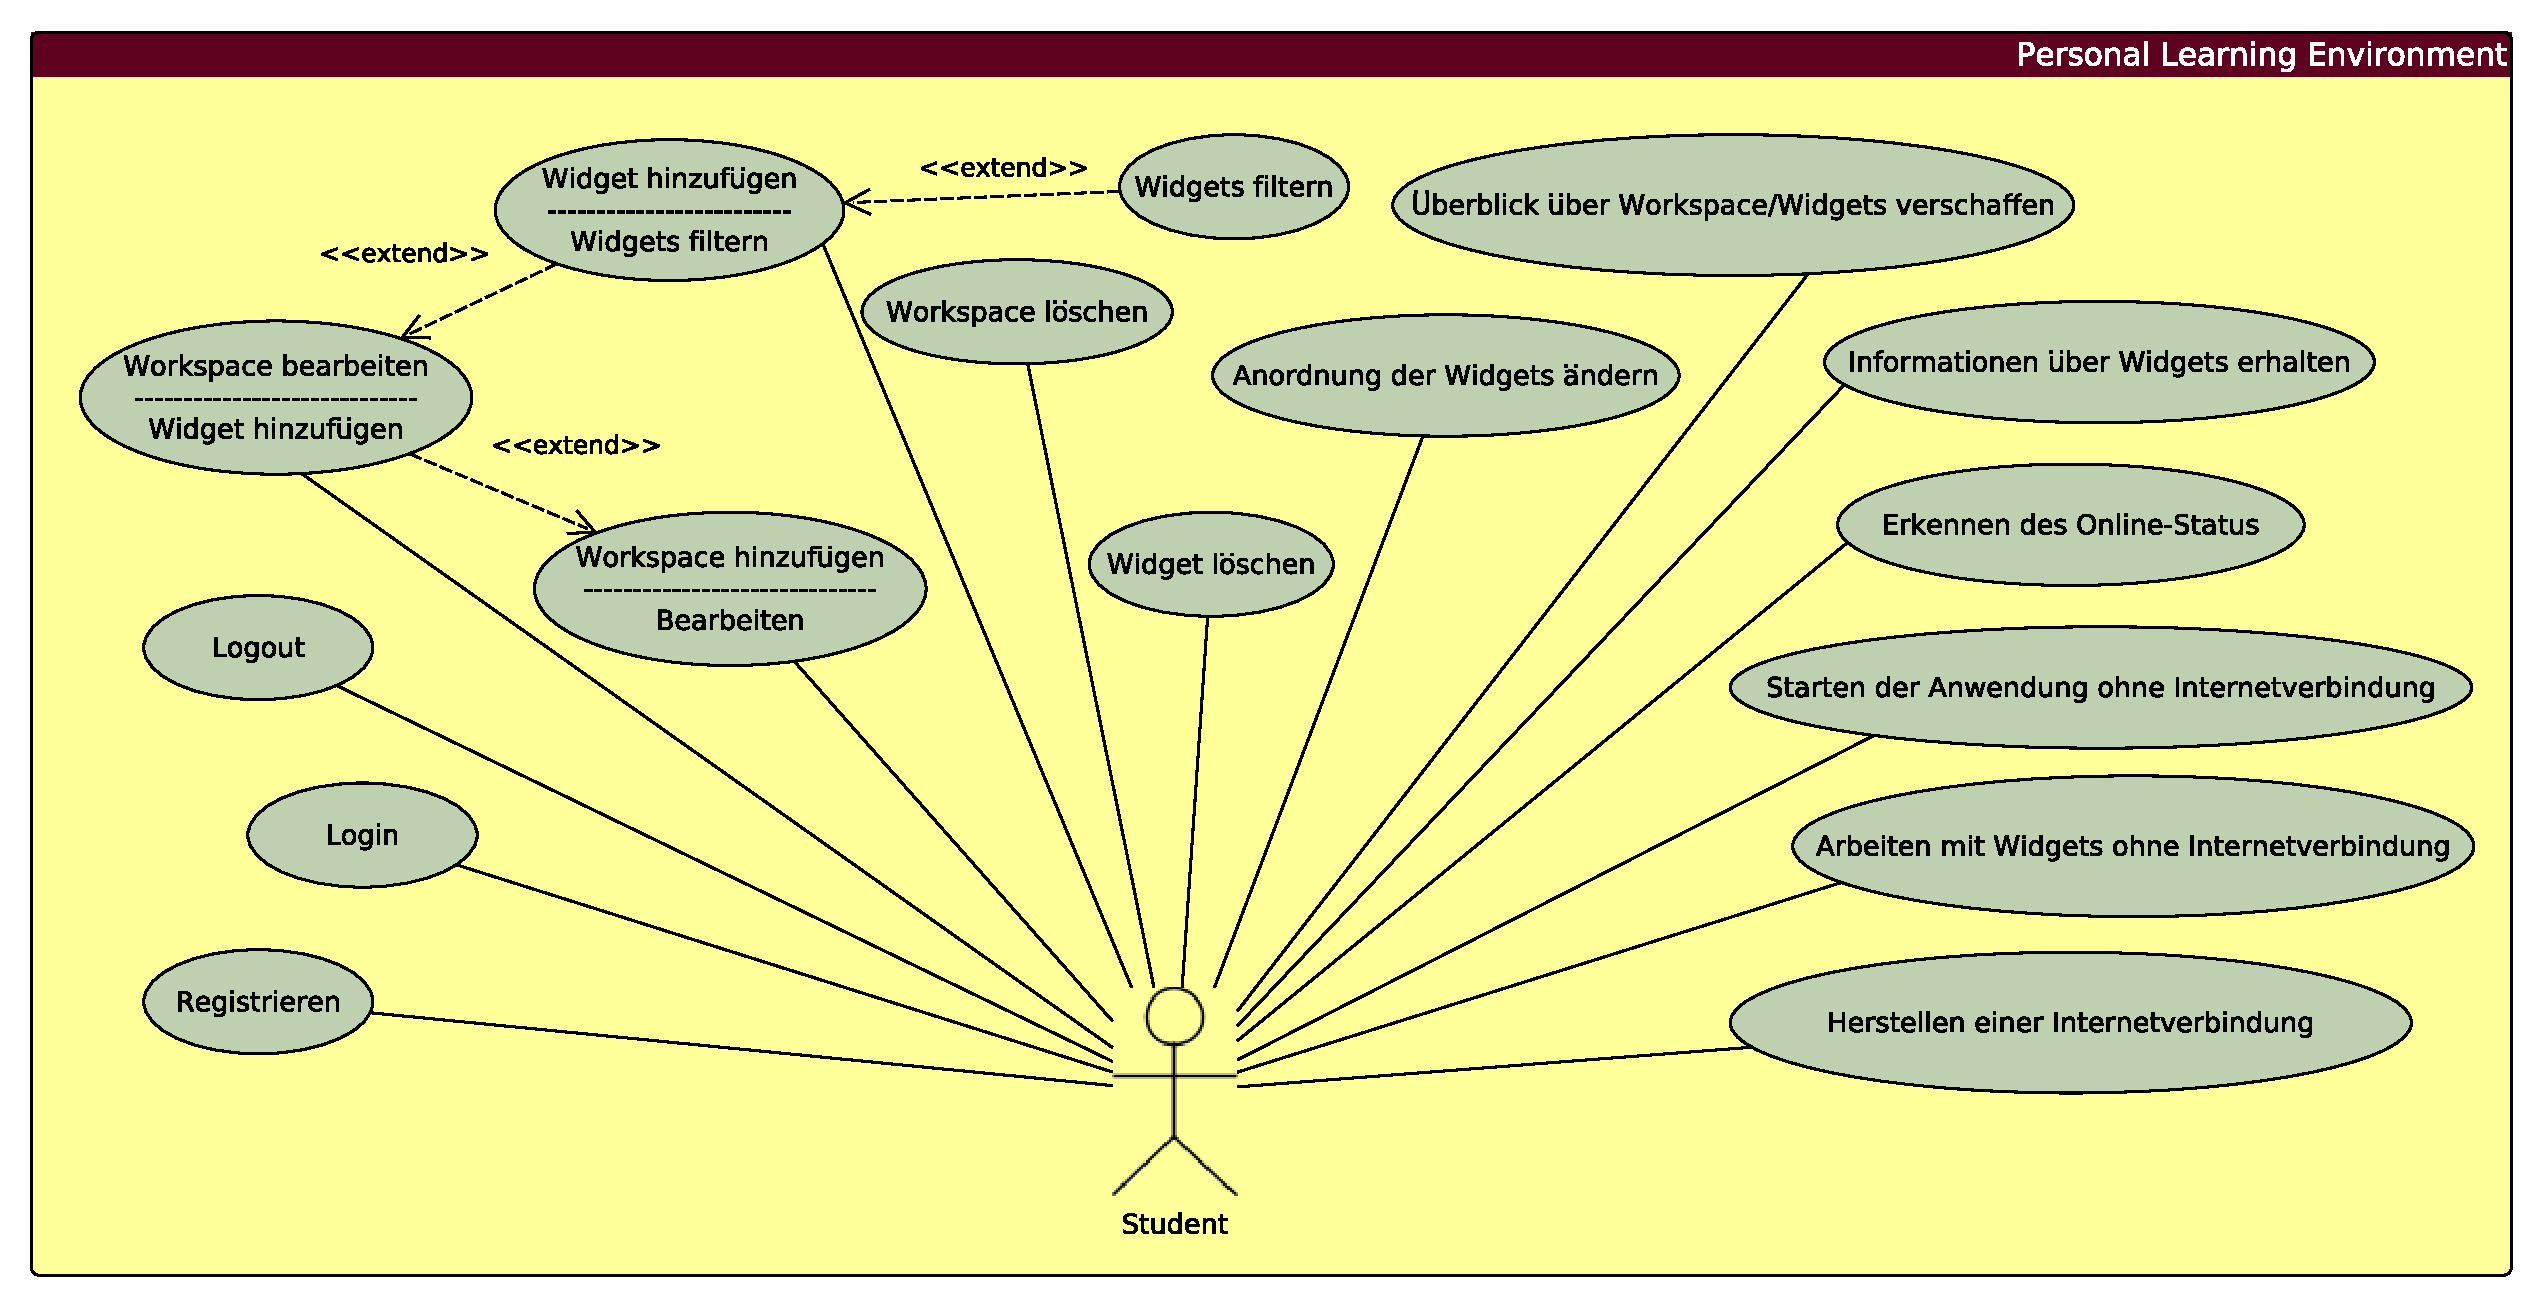
\includegraphics[width=\textwidth,height=\textheight,keepaspectratio]{./Figures/anwendungsfaelle_quer.pdf}
    \rule{35em}{0.5pt}
  \caption[Die wichtigsten Anwendungsfälle für die prototypische Personal Learning EnvironmentAnwendungsfälle der PLE]{Anwendungsfälle der PLE}
  \label{fig:anwendungsfaelle}
\end{figure}

Im folgenden werden die Anwendungsfälle aus Abbildung \ref{fig:anwendungsfaelle} in textueller Form beschrieben. Aus diesen Beschreibungen werden dann direkt die funktionalen Anforderungen an das zu entwickelnde System abgeleitet.

\subsection{Registrieren}
\textbf{use case} \emph{Registrieren}\\
\textbf{actors} Student\\
\textbf{precondition} Das System ist online, der Student ist nicht eingeloggt und es existiert mindestens ein Workspace.\\
\textbf{main flow} Der Student bekommt auf der Startseite die Möglichkeit sich für den Zugang zum System zu registrieren. Er füllt ein Formular mit seinen Daten (Vorname, Nachname, E-Mailadresse, Nutzername, Passwort) aus und schickt das Formular ab.\\
\textbf{postcondition} Der Student ist mit einer Nutzername-/Passwortkombination und seiner E-Mailadresse im System hinterlegt und kann sich somit in das System einloggen.\\
\textbf{exceptional flow} Nutzername oder Mail-Adresse bereits vorhanden. Nutzername und E-Mail-Adresse dürfen nur einmal im System vorkommen.\\
\textbf{postcondition} Der Student bekommt eine Fehlermeldung und muss seine eingetragenen Daten ändern.
 
Aus diesem Anwendungsfall folgt die funktionale Anforderung \emph{fA1}:\\
\emph{fA1: Der Anwender muss sich selbständig in dem registrieren können.}
 
\subsection{Login}
\textbf{use case} \emph{Login}\\
\textbf{actors} Student\\
\textbf{precondition} Das System ist online, der Student ist nicht eingeloggt, ist aber in dem System registriert.\\
\textbf{main flow} Der Student bekommt auf der Startseite die Möglichkeit sich im System anzumelden. Er füllt ein Formular mit seiner Nutzername-/Passwortkombination aus und schickt das Formular ab.\\
\textbf{postcondition} Der Student ist im System eingeloggt und das System präsentiert ihm eine Übersicht über seine aktuellen Workspaces und die wichtigsten aggregierten Informationen dieser.
 
Aus diesem Anwendungsfall folgen die funktionalen Anforderungungen \emph{fA2} und \emph{fA2}:\\
\emph{fA2: Der Anwender muss sich sich in das System mit Nutzername und Passwort einloggen können.}\\
\emph{fA3: Dem Anwender darf nur Zugriff auf die zu seinem Account gehörigen Workspaces und Widgets gewährt werden.}
 
 \subsection{Logout}
\textbf{use case} \emph{Logout}\\
\textbf{actors} Student\\
\textbf{precondition} Das System ist online, der Student ist eingeloggt.\\
\textbf{main flow} Der Student wählt die Aktion "`Logout"' und wird anschließend auf die Login-Seite weitergeleitet.\\
\textbf{postcondition} Die aktuelle Session des Anwenders ist beendet und es ist ohne weiteres Login nicht möglich auf die Daten des Anwenders zuzugreifen 
 
Aus diesem Anwendungsfall folgen die funktionale Anforderung \emph{fA4} und \emph{fA5}:\\
\emph{fA4: Der Anwender muss sich aus dem System ausloggen können.}\\
\emph{fA5: Nach Beendigung der Anwender-Session, darf kein Zugriff mehr auf die Daten des Anwenders bestehen.}
 
\subsection{Workspace hinzufügen}
\textbf{use case} \emph{Workspace hinzufügen}\\
\textbf{actors} Student\\
\textbf{precondition} Das System ist online, der Student ist eingeloggt.\\
\textbf{main flow} Der Student wählt die Aktion "`Workspace hinzufügen"'. Es öffnet sich hierdurch ein neuer Bereich, welcher einen neuen Workspace repräsentiert. Der Student hat nun die Möglichkeit den Workspace nach seinen Wünschen anzupasssen (extension point: Workspace bearbeiten).\\
\textbf{postcondition} Ein neuer Workspace wurde dem System des Studenten hinzugefügt.
 
Aus diesem Anwendungsfall folgt die funktionale Anforderungung \emph{fA6}:\\
\emph{fA6: Der Anwender muss neue Workspaces in seine Lernumgebung einfügen können.}\\
 
\subsection{Workspace bearbeiten}
\textbf{use case} \emph{Workspace bearbeiten}\\
\textbf{actors} Student\\
\textbf{precondition} Das System ist online, der Student ist eingeloggt und es existiert mindestens ein Workspace.\\
\textbf{main flow} Der Student wählt bei einem Workspace die Aktion "`Workspace bearbeiten"'. Der Anwender hat nun die Möglichkeit den Workspace nach seinen Wünschen zu benennen und kann Widgets zu dem Workspace hinzufügen (extension point: Widget hinzufügen).\\
\textbf{postcondition} Der Workspace wurde nach den Vorstellungen des Akteures angepasst.
 
\textbf{extend relationship}\\
\textbf{base} "`Workspace hinzufügen"'\\
\textbf{extensionPoint} Workspace bearbeiten\\
\textbf{extension} "`Workspace bearbeiten"'
 
Aus diesem Anwendungsfall folgt die funktionale Anforderungung \emph{fA7}:\\
\emph{fA7: Der Anwender muss den Namen des Workspaces ändern können.}\\
 
 \subsection{Workspace löschen}
\textbf{use case} \emph{Workspace löschen}\\
\textbf{actors} Student\\
\textbf{precondition} Das System ist online, der Student ist eingeloggt und es existiert mindestens ein Workspace.\\
\textbf{main flow} Der Student wählt bei einem Workspace die Aktion "`Workspace löschen"'. Es erscheint eine Rückfrage, welche eine Bestätigung des Löschvorganges (mitsamt aller Widgets) erfragt. Bei positiver Rückmeldung gibt das System die Nachricht des Löschens aus. \\
\textbf{postcondition} Der Workspace und alle seine Widgets sind aus dem System entfernt.
 
Aus diesem Anwendungsfall folgt die funktionale Anforderungung \emph{fA8}:\\
\emph{fA8: Der Anwender muss einen Workspace löschen können.}\\

\subsection{Widget hinzufügen}
\textbf{use case} \emph{Widget hinzufügen}\\
\textbf{actors} Student\\
\textbf{precondition} Das System ist online, der Student ist eingeloggt und es existiert mindestens ein Workspace.\\
\textbf{main flow} Der Student befindet sich in einem Workspace und wählt die Aktion "`Widget hinzufügen"' Es erscheint eine Maske in der die zur Verfügung stehenden Widgets ausgewählt werden können. Der Student wählt das gewünschte Widget und fügt es dem Workspace hinzu. Wenn gewünscht kann der Student die Liste der Widgets über Suchfilter einschränken (extension point: Widgets filtern)\\
\textbf{postcondition} Das Widget wurde dem Workspace hinzugefügt.
 
\textbf{extend relationship}\\
\textbf{base} `Workspace bearbeiten"'\\
\textbf{extensionPoint} Widget hinzufügen\\
\textbf{extension} "`Widget hinzufügen"'

Aus diesem Anwendungsfall folgt die funktionale Anforderungung \emph{fA9}:\\
\emph{fA9: Der Anwender muss über ein Auswahlfeld Widgets zu Workspaces hinzufügen können.}\\ 

\subsection{Widgets Filtern}
\textbf{use case} \emph{Widgets Filtern}\\
\textbf{actors} Student\\
\textbf{precondition} Der Student ist dabei einem Workspace ein Widget hinzuzufügen.\\
\textbf{main flow} Der Student gibt in einem Textfeld eine Zeichenkette an, nach der im Widgetnamen gesucht wird. Des weiteren kann er in einem binären Filter wählen, ob er nur Widgets angezeigt bekommen möchte, die in der Lage sind in einem Offline-Modus zu arbeiten.\\
\textbf{postcondition} In der Liste der zur Auswahl stehenden Widgets werden nur noch diejenigen angezeigt, die der Filterung entsprechen.
 
\textbf{extend relationship}\\
\textbf{base} "`Widget hinzufügen"'\\
\textbf{extensionPoint} Widgets filtern\\
\textbf{extension} "`Widgets filtern"'
 
Aus diesem Anwendungsfall folgen die funktionalen Anforderungen \emph{fA10} und \emph{fA11}:\\
\emph{fA10: Der Anwender muss die zur Auswahl stehenden Widgets über ein Suchfeld einschränken können.}\\
\emph{fA11: Der Anwender muss die zur Auswahl stehenden Widgets so einschränken können, dass in der Liste nur offline-fähige Widgets vorkommen.}
 
 \subsection{Widget löschen}
\textbf{use case} \emph{Widget löschen}\\
\textbf{actors} Student\\
\textbf{precondition} Das System ist online, der Student ist eingeloggt, er und es existiert mindestens ein Widget auf einem Workspace.\\
\textbf{main flow} Der Student befindet sich in einem Workspace und wählt bei einem Widget die Aktion "`Widget löschen"'. Es erscheint eine Rückfrage, welche eine Bestätigung des Löschvorganges erfragt. Bei positiver Rückmeldung gibt das System die Nachricht des Löschens aus.
\textbf{postcondition} Das Widget wurde aus dem System entfernt.
 
Aus diesem Anwendungsfall folgt die funktionale Anforderungung \emph{fA12}:\\
\emph{fA12: Der Anwender muss ein Widget löschen können.}\\
 
\subsection{Anordnung der Widgets ändern}
\textbf{use case} \emph{Anordnung der Widgets ändern}\\
\textbf{actors}Student\\
\textbf{precondition} Das System ist online, der Student ist eingeloggt und befindet sich auf der Seite eines Workspaces mit mindestens zwei Widgets.\\
\textbf{main flow} Der Student hat die Möglichkeit die einzelnen Widgets innerhalb eines Workspaces über einen Drag and Drop Mechanismus neu anzuordnen. Er wählt hierfür ein Widget mit der Maus aus und zieht es an die gewünschte Position.\\
\textbf{postcondition} Die Anordnung der Widgets innerhalb des Workspaces hat sich nach dem Wunsch des Studenten geändert.
 
Aus diesem Anwendungsfall folgt die funktionale Anforderungung \emph{fA13}:\\
\emph{fA13: Der Anwender muss in der Lage sein Widgets nach seinen Wünschen über einen Drag and Drop Mechanismus auf dem Workspace zu sortieren .}\\
 
\section{Nichtunktionale Anforderungen}\label{section:nichtfunktionale_anforderunge}

\subsection{Voraussetzungen}
Wie in Kapitel \ref{chapter:Kapitel2} beschrieben sind Personal Learning Environments Mashup-Anwendungen, welche unterschiedliche Anwendungen zu einem System zusammenfassen. Diese Anwendungen sind Services oder Kanäle, wie zum Beispiel Twitter, Facebook oder auch Applikationen für Todo-Listen oder Chats. Das System muss also als Aggregator fungieren, welcher diese Anwendungen in einer Anwendung bündelt und dem Nutzer in übersichtlicher Form präsentiert und ihm die Arbeit mit ihnen ermöglicht. Die in den funktionalen Anforderungen beschriebenen Widgets stellen hierbei die Umsetzung dieser Applikationen in der PLE dar. Dem Nutzer sollten genügend Services für seine PLE zur Verfügung stehen und die Entwicklung sollte nicht von einer Person oder Firma abhängen. Aus diesem Grund muss für die Einbindung der Services ein frei verfügbarer Standard und keine proprietäre Schnittstelle verwendet werden.

Somit ergeben sich die nichtfunktionalen Anforderungen \emph{nfA1}, und \emph{nfA2}:\\
\emph{nfA1: Das System muss als Aggregator für unterschiedliche externe Kanäle und Services dienen und dem Anwender die Arbeit mit ihnen an zentraler Stelle ermöglichen.}\\
\emph{nfA2. Die Services müssen über einen frei verfügbaren Standard in das System eingebunden werden können.}

\subsection{Randbedingungen}
Eine wichtige Randbedingung an das System ist der mögliche Einsatz in im Bezug auf die technologische Infrastruktur schwächeren Ländern wie Kamerun. Studenten in solchen Ländern  haben das Problem, dass der Internetzugriff aus mehreren Gründen nicht immer gegeben ist. Es ist beispielsweise möglich, dass sie an ihrem Wohnort keinen Internetzugang besitzen, sondern nur die Möglichkeit haben in der Universität oder in einem Internetcafe online zu gehen. Des weiteren kann ein vorhandener Internetzugang relativ langsam sein und nach Zeit abgerechnet werden, so dass es vorteilhaft ist, nur für kurze Zeit online zu sein. Aus diesen Gründen wird eine System benötigt, welches die Möglichkeit bietet die neuesten Informationen auch offline zu lesen und zumindest rudimentär offline kleine Aufgaben zu erledigen. Diese sollten sich bei Wiederverbindung mit dem Internet mit den entsprechenden Services synchronisieren. Die Möglichkeit der Offlinebenutzbarkeit des Systems spielt auch für die Verwendung auf aktuellen mobilen Geräten wie Smartphones oder Tablets eine wichtige Rolle. Eine Internetverbindung ist auch hier nicht immer gewährleistet oder sie kann temporär deaktiviert werden, um die Akkulaufzeit der Geräte zu verlängern. 
Zusätzlich sollten die die Daten auch ohne Internetverbindung zwischen verschiedenen Rechnern ausgetauscht werden können, so dass gewisse Arbeiten an einem Rechner durchgeführt werden können und diese Arbeiten dann an einem Rechner mit Internetanschluss zu synchronisieren.
Somit ergeben sich die nichtfunktionalen Anforderungen \emph{nfA3}, und \emph{nfA4}:\\
\emph{nfA3: Das System muss den Anwender in die Lage versetzen mit den gewählten Services, zumindest rudimentär, offline zu arbeiten. Bei einer Verbindung mit dem Internet müssen die vorgenommenen Arbeiten synchronisiert werden.}\\
\emph{nfA4: Die durchgeführten Arbeiten müssen offline zwischen unterschiedlichen Rechnern transportiert werden können.}

Dadurch, dass die Studenten an unterschiedlichen Rechnern mit potentiell unterschiedlichen Betriebssystemen, arbeiten, welche zum Teil nicht in ihrem persönlichen Besitz sind, ist es für sie nicht oder nur sehr schwer möglich eine neue Software zu installieren. Aus diesem Grund soll das System mit nativen Browsertechnologien ohne weitere Installation nutzbar sein:\\
\emph{nfA5: Das System muss in aktuellen Browsern mit nativen Browsertechnologien ohne weitere Installation nutzbar sein.}

\subsection{Erweiterbarkeit}
In dieser Arbeit kann nur eine prototypische Implementierung der Anforderungen erfolgen. Das System soll also als Basis für weitere Entwicklungen und Forschungsarbeiten dienen und einfach erweitert und verändert werden können. Das System muss als Aggregator für die unterschiedlichsten Services dienen. Es soll aus diesem Grund möglich sein auf Basis einer vorgegebenen Implementierung oder API weitere Services oder Kanäle in das System zu laden, welche ebenfalls offlinefähig sind und es so beständig in seiner Funktionalität zu erweitern. Schließlich wird die Software in unterschiedlichen Bereichen, insbesondere in einem universitären Umfeld eingesetzt. Dies verlangt eine Nutzbarkeit ohne Lizengebühren für die verwendeten Technologien, so dass für die Umsetzung keine proprietären, sondern nur freie Technologien verwendet werden dürfen. Aus diesen Punkten folgen die nichtfunktionalen Anforderungen \emph{nfA6}, \emph{nfA7} und \emph{nfA8}:\\
\emph{nfA6: Das System muss einfach erweitert werden können.}\\
\emph{nfA7: Es muss möglich sein über eine API oder eine vorgegebene Implementierung neue Services und Kanäle mit Offlinefähigkeiten in das System zu laden.}\\
\emph{nfA8: Es dürfen keine proprietären, sondern nur freie Technologien für die Umsetzung des Systems genutzt werden.}

 
\section{Überblick über die Anforderungen}
Im den vorherigen Abschnitten wurden funktionale und nichtfunktionale Anforderungen an das zu entwickelnde System aufgestellt und beschrieben. In den folgenden zwei Tabellen sind diese Anforderungen noch einmal zusammengefasst.

\begin{table}[h]
\caption{Funktionale Anforderungen}
\begin{tabularx}{\textwidth}{ l | X }
\emph{fA1} & \emph{Der Anwender muss sich selbständig in dem registrieren können.} \\ \hline
\emph{fA2} & \emph{Der Anwender muss sich sich in das System mit Nutzername und Passwort einloggen können.} \\ \hline
\emph{fA3} & \emph{Dem Anwender darf nur Zugriff auf die zu seinem Account gehörigen Workspaces und Widgets gewährt werden.} \\ \hline
\emph{fA4} & \emph{Der Anwender muss sich aus dem System ausloggen können.} \\ \hline
\emph{fA5} & \emph{Nach Beendigung der Anwender-Session, darf kein Zugriff mehr auf die Daten des Anwenders bestehen.} \\ \hline
\emph{fA6} & \emph{Der Anwender muss neue Workspaces in seine Lernumgebung einfügen können.} \\ \hline
\emph{fA7} & \emph{Der Anwender muss den Namen des Workspaces ändern können.} \\ \hline
\emph{fA8} & \emph{Der Anwender muss einen Workspace löschen können.} \\ \hline
\emph{fA9} & \emph{Der Anwender muss über ein Auswahlfeld Widgets zu Workspaces hinzufügen können.} \\ \hline
\emph{fA10} & \emph{Der Anwender muss die zur Auswahl stehenden Widgets über ein Suchfeld einschränken können.} \\ \hline
\emph{fA11} & \emph{Der Anwender muss die zur Auswahl stehenden Widgets so einschränken können, dass in der Liste nur offline-fähige Widgets vorkommen.} \\ \hline
\emph{fA12} & \emph{Der Anwender muss ein Widget löschen können.} \\\hline
\emph{fA13} & \emph{Der Anwender muss in der Lage sein Widgets nach seinen Wünschen über einen Drag and Drop Mechanismus auf dem Workspace zu sortieren .} \\ \hline
\end{tabularx}
\label{table:funktionale_anforderungen}
\end{table}

\renewcommand{\arraystretch}{1.4} 
\begin{table}[h]
\caption{Nichtfunktionale Anforderungen}
\begin{tabularx}{\textwidth}{ l | X }
\emph{nfA1} & \emph{Das System muss als Aggregator für unterschiedliche externe Kanäle und Services dienen und dem Anwender die Arbeit mit ihnen an zentraler Stelle ermöglichen.} \\ \hline
\emph{nfA2} & \emph{Die Services müssen über einen frei verfügbaren Standard in das System eingebunden werden können.} \\ \hline
\emph{nfA3} & \emph{Das System muss den Anwender in die Lage versetzen mit den gewählten Services, zumindest rudimentär, offline zu arbeiten. Bei einer Verbindung mit dem Internet müssen die vorgenommenen Arbeiten synchronisiert werden.} \\ \hline
\emph{nfA4} & \emph{Die durchgeführten Arbeiten müssen offline zwischen unterschiedlichen Rechnern transportiert werden können.} \\ \hline
\emph{nfA5} & \emph{Das System muss in aktuellen Browsern mit nativen Browsertechnologien ohne weitere Installation nutzbar sein.} \\ \hline
\emph{nfA6} & \emph{Das System muss einfach erweitert werden können.} \\ \hline
\emph{nfA7} & \emph{Es muss möglich sein über eine API oder eine vorgegebene Implementierung neue Services und Kanäle mit Offlinefähigkeiten in das System zu laden.} \\ \hline
\emph{nfA8} & \emph{Es dürfen keine proprietären, sondern nur freie Technologien für die Umsetzung des Systems genutzt werden.} \\ \hline
\end{tabularx}
\label{table:nichtfunktionale_anforderungen}
\end{table}
